\documentclass{article}

\usepackage[utf8]{inputenc}
\usepackage[ngerman]{babel}
\usepackage[ngerman]{translator}
\usepackage[T1]{fontenc}
\usepackage{enumitem}
\usepackage{graphicx}
\usepackage{float}
\usepackage{url}
\usepackage[bottom]{footmisc}
\usepackage{hyperref}
\usepackage[nonumberlist, section=subsection]{glossaries}

\title{\textbf{Entwurf} \\ Cryptographics}
\author{}
\date{\today}

%Glossar-Befehle anschalten
\makeglossaries
% \newglossaryentry{identifier}{name={Name}, description={Description}}

\begin{document}

% The cover page.
\maketitle
\begin{table}[b]
  \begin{tabular}{| l | l | l |}
    \hline
    \textbf{Phase} & \textbf{Verantwortlicher} & \textbf{Email} \\ \hline
    Pflichtenheft & Matthias Jaenicke & matthias.jaenicke@student.kit.edu \\ \hline
    Entwurf & Matthias Plappert & undkc@student.kit.edu \\
            & Julien Duman & uncyc@student.kit.edu \\ \hline
    Implementierung & Christian Dreher & uaeef@student.kit.edu \\ \hline
    Qualitätssicherung & Wasilij Beskorovajnov & uajkm@student.kit.edu \\ \hline
    Präsentation & Aydin Tekin & aydin.tekin@student.kit.edu \\ \hline
    \end{tabular}
\end{table}
\thispagestyle{empty}
\newpage

% Table of contents page.
\tableofcontents
\newpage

% Start of the actual document.
\section{Einleitung}
Für das Kryptologikum des Instituts für Kryptographie und Sicherheit soll die Software Cryptographics zur Demonstration kryptographischer Verfahren erstellt werden. Das Softwareprodukt soll vor allem auf Ausstellungen präsentiert werden und erfordert daher eine möglichst intuitive Benutzerführung.

Um das Ziel der intuitiven Benutzerinteraktion zu erreichen, liegt das Hauptaugenmerk des Entwurfes auf der Planung eines Rahmenwerkes, dass es erlaubt, einzelne Verfahren in die Software einzubetten. Durch wiederverwendbare UI-Komponenten sowie eine einheitliche und für alle Verfahren identischen Benutzerführung erreichen wir dieses Ziel. Zusätzlich erlaubt uns dieser Entwurf, wiederkehrende Aufgaben wie beispielsweise die Soforthilfe mit minimalem Aufwand innerhalb der einzelnen Verfahren zu implementieren. Die eigentliche Komplexität steckt hierbei immer im Rahmenwerk, sodass alle Verfahren von Verbesserungen und Optimierungen profitieren. Weiterhin setzen wir auf eine simples, modulares System, dass es uns erlaubt, Verfahren mit minimalem Aufwand zu implementieren, zu warten und auszutauschen. Grundprinzipien ist hierbei die lose Kopplung der einzelnen Verfahren.

Eine Herausforderung stellte die Abwägung zwischen Konsistenz und einer nötigen Flexibilität innerhalb der Verfahren da. So erfordern beispielsweise unterschiedliche Verfahren durchaus sehr unterschiedliche Arten der Navigation. Unser Entwurf sieht hierbei vor, dass die einzelnen Verfahren durchaus flexible und ohne strikte Vorgaben funktionieren können, gewisse Funktionen wie beispielsweise die Hilfe immer auf dieselbe Art funktionieren. Das oben beschriebene Rahmenwerk agiert auch hier unterstützend, erlaubt aber eine gewisse Flexibilität beispielsweise bei der Navigation innerhalb des Verfahrens. Somit lassen sich eine Vielzahl von unterschiedlichen Visualisierungen realisieren.

\section{Aufbau}

\subsection{Architektur}

Die grundlegende Architektur gliedert sich in 4 Schichten. Hierbei implementieren die Schichten von unten nach oben Funktionalität, die dann in der höheren Schicht verwendet werden kann.

\begin{figure}[H]
  \centering
    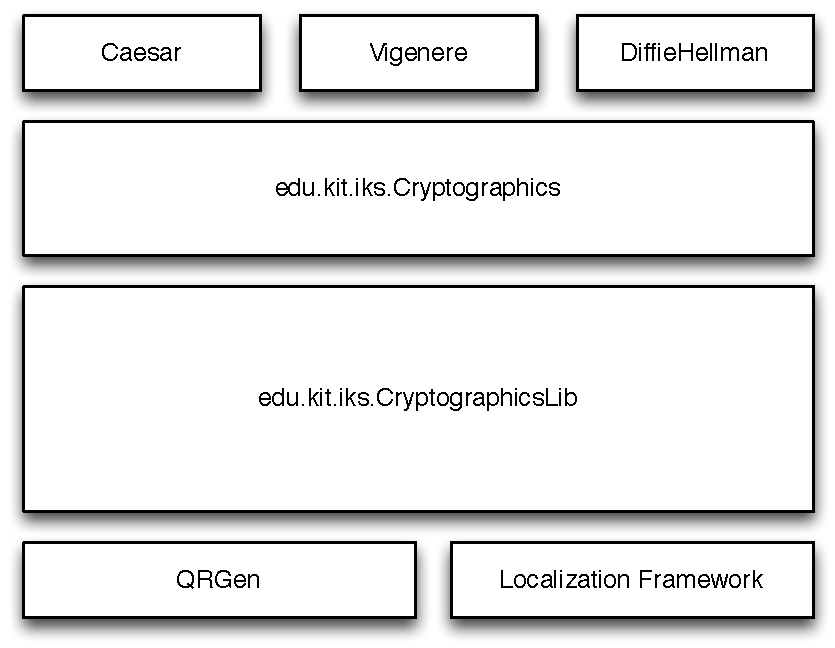
\includegraphics[width=\textwidth]{resources/architecture}
  \caption{Architekturübersicht.}
\end{figure}

In der ersten, der untersten Schicht befinden sich Bibliotheken von Drittanbietern. In unserem Fall handelt es sich hierbei um QRGen, eine Java-Bibliothek um QR-Codes zu generieren, sowie um ein Framework zur Lokalisierung.

In der zweiten Schicht befindet sich das Modul edu.kit.iks.CryptographicsLib. Dieses Modul enthält zum Einen abstrakte Klassen, die von den weiter oben liegenden Klassen verwendet werden. Zum Anderen finden sich hier wiederverwendbare UI-Komponenten, die beispielsweise bei verschiedenen Verfahren verwendet werden können.

Die dritte Schicht besteht aus dem Modul edu.kit.iks.Cryptographics. Hierbei handelt es sich um das Rahmenwerk, in dem alle Visualisierungen ausgeführt werden. Hier wird beispielsweise die Logik implementiert um zwischen Verfahren über eine Zeitleiste wechseln zu können oder auch die Soforthilfe.

Die oberste und vierte Schicht besteht aus den einzelnen, konkreten Verfahren.

Alle Schichten unterteilen ihre Klassen nach dem Model-View-Controller-Prinzip um eine Trennung von Datenmodell, Präsentation und Programmsteuerung zu erreichen. Sowohl die Präsentation als auch die Programmsteuerung verwendet hierbei das Entwurfsmuster Kompositum. Dies erlaubt es uns, eine hierarchische Struktur zu implementieren, und die Aufgaben der Programmsteuerung klar voneinander abzugrenzen. Eine schematische Darstellung der Controller-Hierarchie während einer Visualisierung ist in Abb. 2 zu finden.

\begin{figure}[H]
  \centering
    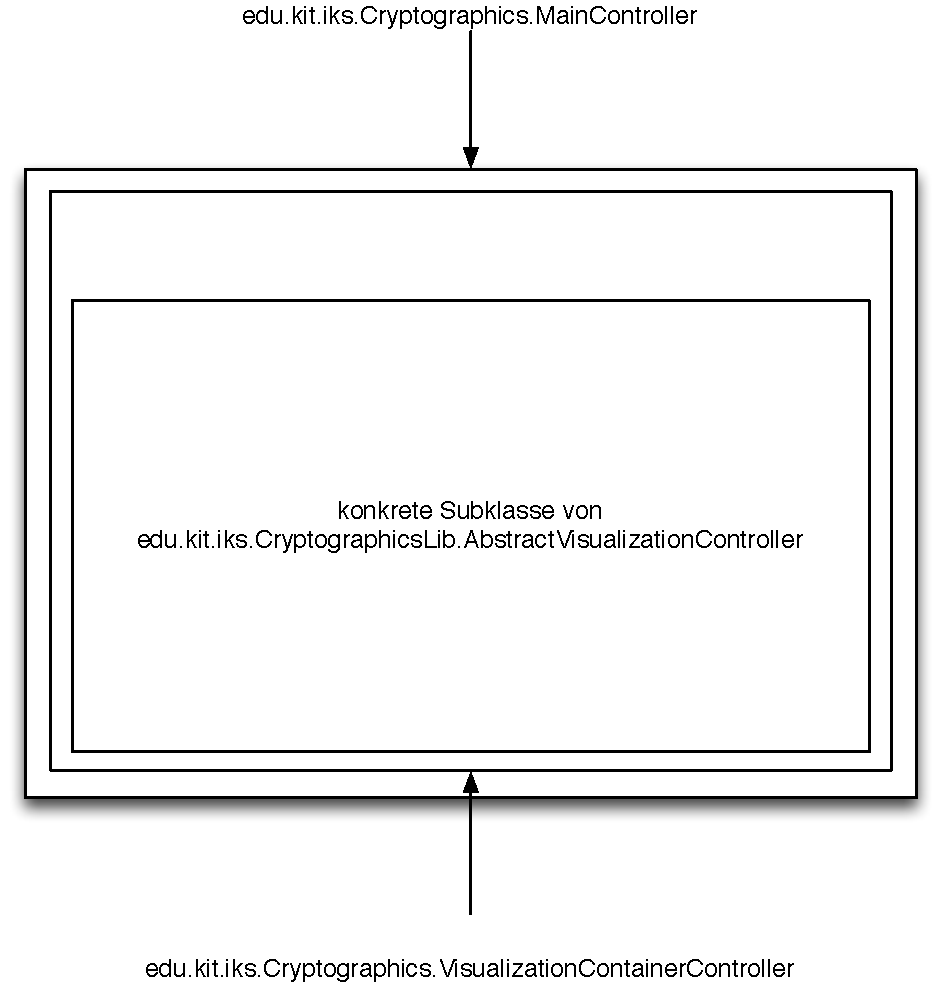
\includegraphics[width=\textwidth]{resources/architecture-2}
  \caption{Darstellung der einzelnen Controller während einer Visualisierung.}
\end{figure}

\section{Klassenbeschreibung}
  \subsection{Paket edu.kit.iks.Cryptographics}
    \subsubsection{Klasse HelpPopoverView}
      Die HelpPopoverView stellt bei Bedarf die Soforthilfe dar.
      \begin{figure}[H]
        \centering
        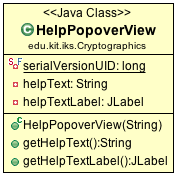
\includegraphics{resources/edu-kit-iks-Cryptographics-HelpPopoverView}
      \end{figure}

      \textbf{Superklassen und Interfaces}
      \begin{itemize}
        \item edu.kit.iks.CryptographicsLib.PopoverView
      \end{itemize}
      
      \textbf{Methoden}
      \begin{itemize}
        \item public HelpPopoverView(String helpText) \newline
        Konstruktor. Erstellt eine HelpPopoverView mit einem gegebenen Hilfstext.
      \end{itemize}

      \textbf{Getter}
      \begin{itemize}
        \item public String getHelpText() \newline
        Gibt den im Konstruktor übergebenen Hilfstext zurück.
        \item public String getHelpTextLabel() \newline
      \end{itemize}

      \textbf{Setter}
      \begin{itemize}
        \item \textit{keine}
      \end{itemize}

    \subsubsection{Klasse Main}
      Main stellt den Einstiegspunkt des Programmes dar.
      \begin{figure}[H]
        \centering
        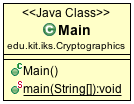
\includegraphics{resources/edu-kit-iks-Cryptographics-Main}
      \end{figure}

      \textbf{Superklassen und Interfaces}
      \begin{itemize}
        \item \textit{keine}
      \end{itemize}
      
      \textbf{Methoden}
      \begin{itemize}
        \item public static void main(String[] args) \newline
        Initialisiert den MainController.
      \end{itemize}

      \textbf{Getter}
      \begin{itemize}
        \item \textit{keine}
      \end{itemize}

      \textbf{Setter}
      \begin{itemize}
        \item \textit{keine}
      \end{itemize}

    \subsubsection{Klasse MainController}
      Der MainController erzeugt das Fenster und verwaltet Start- und VisualizationContainerController.
      \begin{figure}[H]
        \centering
        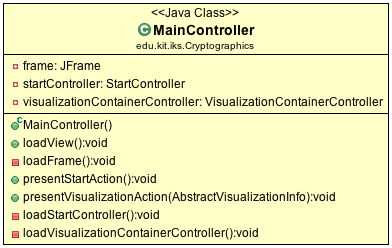
\includegraphics{resources/edu-kit-iks-Cryptographics-MainController}
      \end{figure}

      \textbf{Superklassen und Interfaces}
      \begin{itemize}
        \item edu.kit.iks.CryptographicsLib.AbstractController
      \end{itemize}
      
      \textbf{Methoden}
      \begin{itemize}
        \item public void loadView() \newline
        Lädt die View.
        \item public void presentStartAction() \newline
        Lädt den StartController und zeigt seine View an.
        \item public void presentVisualizationAction(AbstractVisualizationInfo visualizationInfo) \newline
        Lädt den VisualizationContainerController, übergibt die konkrete VisualizationInfo und zeigt seine View an.
      \end{itemize}

      \textbf{Getter}
      \begin{itemize}
        \item \textit{keine}
      \end{itemize}

      \textbf{Setter}
      \begin{itemize}
        \item \textit{keine}
      \end{itemize}

    \subsubsection{Klasse StartController}
      Der StartController verwaltet TimelineView sowie WelcomeView. Weiterhin zeigt er die TimelinePopoverView an und delegiert das Laden eines Verfahrens an den MainController.
      \begin{figure}[H]
        \centering
        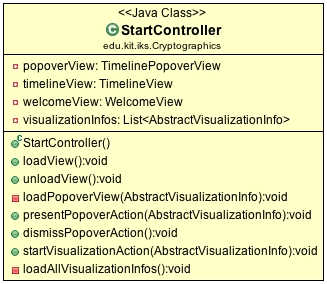
\includegraphics{resources/edu-kit-iks-Cryptographics-StartController}
      \end{figure}

      \textbf{Superklassen und Interfaces}
      \begin{itemize}
        \item edu.kit.iks.CryptographicsLib.AbstractController
      \end{itemize}
      
      \textbf{Methoden}
      \begin{itemize}
        \item public void loadView() \newline
        Lädt die View.
        \item public void unloadView() \newline
        Gibt die View frei.
        \item public void presentPopoverAction(AbstractVisualizationInfon visualizationInfo) \newline
        Erzeugt und präsentiert eine TimelinePopoverView, die Informationen zur gewählten Visualisierung enthält.
        \item public void dismissPopoverAction() \newline
        Entfernt die aktuelle TimelinePopoverView.
        \item public void startVisualizationAction(AbstractVisualizationInfon visualizationInfo) \newline
        Die gewählte Visualisierung soll gestartet werden. Hierzu delegiert diese Methode die Aufgabe an den MainController.
      \end{itemize}

      \textbf{Getter}
      \begin{itemize}
        \item \textit{keine}
      \end{itemize}

      \textbf{Setter}
      \begin{itemize}
        \item \textit{keine}
      \end{itemize}

    \subsubsection{Klasse TimelinePopoverView}
      Die TimelinePopoverView stellt Informationen zu einer gewählten Visualisierung dar und bietet eine Möglichkeit an die Visualisierung zu starten.
      \begin{figure}[H]
        \centering
        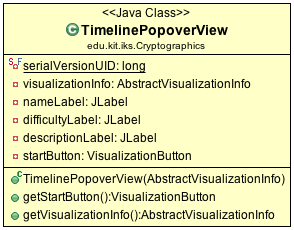
\includegraphics{resources/edu-kit-iks-Cryptographics-TimelinePopoverView}
      \end{figure}

      \textbf{Superklassen und Interfaces}
      \begin{itemize}
        \item edu.kit.iks.CryptographicsLib.PopoverView
      \end{itemize}
      
      \textbf{Methoden}
      \begin{itemize}
        \item public TimelinePopoverView(AbstractVisualizationInfo visualizationInfo) \newline
        Konstruktor. Erzeugt eine neue TimelinePopoverView und übergibt die benötigten Informationen zur Darstellung als AbstractVisualizationInfo.
      \end{itemize}

      \textbf{Getter}
      \begin{itemize}
        \item public VisualizationButton getStartButton()
        \item public AbstractVisualizationInfo getVisualizationInfo()
      \end{itemize}

      \textbf{Setter}
      \begin{itemize}
        \item \textit{keine}
      \end{itemize}

    \subsubsection{Klasse TimelineView}
      Die TimelineView stellt alle Visualisierung auf einer Zeitleiste dar.
      \begin{figure}[H]
        \centering
        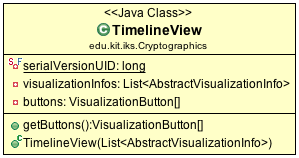
\includegraphics{resources/edu-kit-iks-Cryptographics-TimelineView}
      \end{figure}

      \textbf{Superklassen und Interfaces}
      \begin{itemize}
        \item javax.swing.JPanel
      \end{itemize}
      
      \textbf{Methoden}
      \begin{itemize}
        \item public TimelineView(List<AbstractVisualizationInfo> visualizationInfos) \newline
        Konstruktor. Erzeugt eine neue TimelineView mit einer Liste von Visualisierungen.
      \end{itemize}

      \textbf{Getter}
      \begin{itemize}
        \item public VisualizationButton[] getButtons() \newline
        Gibt alle Buttons der TimelineView zurück. Jeder Button steht für eine Visualisierung auf der Zeitleiste.
      \end{itemize}

      \textbf{Setter}
      \begin{itemize}
        \item \textit{keine}
      \end{itemize}

    \subsubsection{Klasse VisualizationContainerController}
      Der VisualizationContainerController bietet den Rahmen für alle Visualisierungen. Seine Aufgabe ist es, zum einen die Funktionalität der VisualizationContainerView zu implementieren, zum anderen stellt er konkrete Subklassen von AbstractVisualizationController dar. Weiterhin bietet VisualizationContainerController eine Möglichkeit zwischen allen AbstractVisualizationControllern hin- und herzuwechseln.
      \begin{figure}[H]
        \centering
        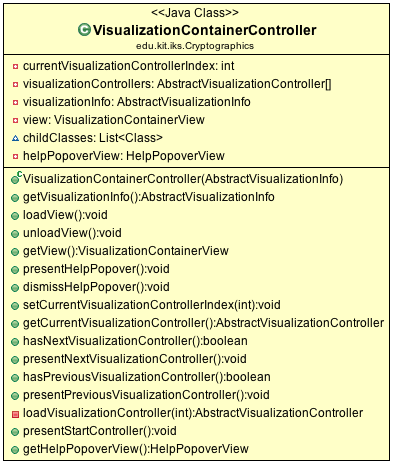
\includegraphics{resources/edu-kit-iks-Cryptographics-VisualizationContainerController}
      \end{figure}

      \textbf{Superklassen und Interfaces}
      \begin{itemize}
        \item edu.kit.iks.CryptographicsLib.AbstractController
      \end{itemize}
      
      \textbf{Methoden}
      \begin{itemize}
        \item public VisualizationContainerController(AbstractVisualizationInfo visualizationInfo) \newline
        Konstruktor. Erzeugt einen neuen VisualizationContainerController für die gegebene Visualisierung.
        Hierbei wird über die übergebene AbstractVisualizationInfo die Liste aller childClasses abgefragt.
        Diese Liste enthält konkrete Klassen, die von AbstractVisualizationController erben und das eigentliche Verfahren schrittweise implementieren.
        \item public void loadView() \newline
        Lädt die View.
        \item public void unloadView() \newline
        Gibt die View frei.
        \item public void presentHelpPopover() \newline
        Zeigt die aktuelle Soforthilfe in einer HelpPopoverView an. Der Hilfstext wird dabei vom aktuellen
        AbstractVisualizationController abgefragt.
        \item public void dismissHelpPopover() \newline
        Entfernt die aktuelle HelpPopoverView.
        \item presentNextVisualizationController() \newline
        Wechselt zum nächsten AbstractVisualizationController aus der Liste der childClasses.
        \item presentPreviousVisualizationController() \newline
        Wechselt zum vorherigen AbstractVisualizationController aus der Liste der childClasses.
        \item presentStartController() \newline
        Delegiert den Wechsel zurück zum StartController an den MainController.
      \end{itemize}

      \textbf{Getter}
      \begin{itemize}
        \item public AbstractVisualizationInfo getVisualizationInfo()
        \item public VisualizationContainerView getView()
        \item public AbstractVisualizationController getCurrentVisualizationContoller() \newline
        Gibt den aktuell verwendeten AbstractVisualizationController zurück.
        \item public boolean hasNextVisualizationController() \newline
        Überprüft, ob es einen nächsten AbstractVisualizationController gibt.
        \item public boolean hasPreviousVisualizationController() \newline
        Überprüft, ob es einen vorherigen AbstractVisualizationController gibt.
        \item public HelpPopoverView getHelpPopoverView() \newline
        Gibt die aktuelle HelpPopoverView zurück falls diese existiert.
      \end{itemize}

      \textbf{Setter}
      \begin{itemize}
        \item setCurrentVisualizationControllerIndex(int index) \newline
        Setzt den aktuellen AbstractViewController auf den in index spezifizierten. Diese Methode läd bei Bedarf 
        die konkrete Instanz aus der Liste childClasses und speichert die Instanz in visualizationControllers.
      \end{itemize}

    \subsubsection{Klasse VisualizationContainerView}
      Die VisualizationContainerView bietet einen Rahmen für die eigentliche Visualisierung. Hierbei wird der Name der Visualisierung sowie zwei Buttons um die Visualisierung abzubrechen sowie die Soforthilfe aufzurufen dargestellt.
      \begin{figure}[H]
        \centering
        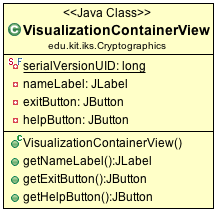
\includegraphics{resources/edu-kit-iks-Cryptographics-VisualizationContainerView}
      \end{figure}

      \textbf{Superklassen und Interfaces}
      \begin{itemize}
        \item javax.swing.JPanel
      \end{itemize}
      
      \textbf{Methoden}
      \begin{itemize}
        \item \textit{keine}
      \end{itemize}

      \textbf{Getter}
      \begin{itemize}
        \item public JLabel getNameLabel()
        \item public JLabel getExitButton()
        \item public JLabel getHelpButton()
      \end{itemize}

      \textbf{Setter}
      \begin{itemize}
        \item \textit{keine}
      \end{itemize}

    \subsubsection{Klasse WelcomeView}
      Die WelcomeView wird oberhalb der TimelineView im StartController dargestellt und begrüßt den Benutzer.
      \begin{figure}[H]
        \centering
        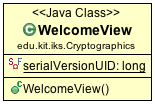
\includegraphics{resources/edu-kit-iks-Cryptographics-WelcomeView}
      \end{figure}

      \textbf{Superklassen und Interfaces}
      \begin{itemize}
        \item javax.swing.JPanel
      \end{itemize}
      
      \textbf{Methoden}
      \begin{itemize}
        \item \textit{keine}
      \end{itemize}

      \textbf{Getter}
      \begin{itemize}
        \item \textit{keine}
      \end{itemize}

      \textbf{Setter}
      \begin{itemize}
        \item \textit{keine}
      \end{itemize}

  \subsection{Paket edu.kit.iks.CryptographicsLib}
    
    % AbstractController
  	\subsubsection{Klasse AbstractController}
	  Um die MVC-Architektur zu erleichtern wird ein abstrakter Controller benötigt, mit dem Mechanismen
	  für die Controller ausgelagert werden können. Des Weiteren bietet das die Möglichkeit, konkrete
	  Controller mit Hilfe ihrer Substitution anzusprechen.
	
      \begin{figure}[H]
        \centering
        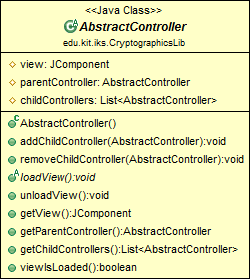
\includegraphics{resources/edu-kit-iks-CryptographicsLib-AbstractController}
      \end{figure}
	
      \textbf{Superklassen und Interfaces}
      \begin{itemize}
        \item \textit{keine}
      \end{itemize}
	
      \textbf{Methoden}
      \begin{itemize}
        \item public void addChildController(AbstractController childController) \newline
          Fügt den übergebenen Kind-Controller zur Liste der Kind-Controller hinzu.
        
        \item public void removeChildController(AbstractController childController) \newline
          Entfernt den übergebenen Kind-Controller aus der Liste der Kind-Controller.
          
        \item abstract public void loadView() \newline
          Abstrakte Deklaration der loadView()-Methode zwingt die erbenden Controller dazu,
          zu definieren, wie ihre View geladen werden soll.
          
        \item public void unloadView() \newline
          Gibt den von der View verbrauchten Speicher wieder frei, sofern diese nicht mehr
          benötigt wird. Zu beachten ist, dass diese Methode über eine Standardimplementierung
          verfügt, es aber durchaus sinnvoll sein kann, das Standardverhalten durch eine
          eigene Implementierung zu überschreiben.
        
        \item public boolean viewIsLoaded() \newline
          Prüft ab, ob die View bereits geladen ist oder nicht.
      \end{itemize}
      
      \textbf{Getter}
      \begin{itemize}
        \item public JComponent getView()
        \item public AbstractController getParentController()
        \item public List<AbstractController> getChildControllers()
      \end{itemize}
      
      \textbf{Setter}
      \begin{itemize}
        \item \textit{keine}
      \end{itemize}
	% /AbstractController
	
	% AbstractVisualizationController
	\subsubsection{Klasse AbstractVisualizationController}
	  Diese abstrakte Klasse konkretisiert den AbstractController zur Verwendung als
	  abstrakter Controller speziell für Visualisierungen. Dies umfasst unter anderem
	  ein Konstruktor, der eine VisualizationInfo als Parameter übergeben bekommt und
	  sich damit initialisiert, sowie einige für Visualisierungen gemeinsame Methoden.
	
      \begin{figure}[H]
        \centering
        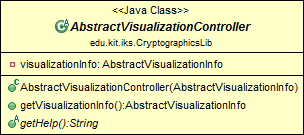
\includegraphics{resources/edu-kit-iks-CryptographicsLib-AbstractVisualizationController}
      \end{figure}
	
      \textbf{Superklassen und Interfaces}
      \begin{itemize}
        \item edu.kit.iks.CryptographicsLib.AbstractController
      \end{itemize}
	
      \textbf{Methoden}
      \begin{itemize}
        \item public AbstractVisualizationController(AbstractVisualizationInfo visualizationInfo) \newline
          Konstruktor. Bekommt als Parameter eine VisualizationInfo, die als Attribut gehalten wird.
        \item abstract public String getHelp() \newline
          Durch das Implementieren dieser Schnittstelle innerhalb eines konkreten Visualisierungs-Controllers
          soll eine einheitliche Hilfe-Funktion geschaffen werden. Dabei muss der konkrete Visualisierungs-
          Controller selbst entscheiden, was die aktuell passende Hilfe ist.
      \end{itemize}
      
      \textbf{Getter}
      \begin{itemize}
		\item public AbstractVisualizationInfo getVisualizationInfo()
      \end{itemize}
      
      \textbf{Setter}
      \begin{itemize}
        \item \textit{keine}
      \end{itemize}
	% /AbstractVisualizationController
	
	% AbstractVisualizationInfo
	\subsubsection{Klasse AbstractVisualizationInfo}
	  Um mit den Metadaten der einzelnen Visualisierungen besser umgehen zu können
	  wird diese Klasse benötigt. Eine konkrete VisualizationInfo muss des Weiteren
	  die abstrakten Methoden implementieren und wird so dazu gezwungen, die 
	  benötigten Metadaten einer Visualisierung bereitzustellen.
	
      \begin{figure}[H]
        \centering
        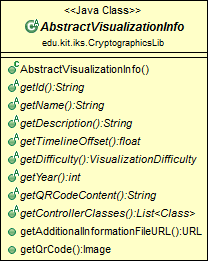
\includegraphics{resources/edu-kit-iks-CryptographicsLib-AbstractVisualizationInfo}
      \end{figure}
	
      \textbf{Superklassen und Interfaces}
      \begin{itemize}
        \item \textit{keine}
      \end{itemize}
	
      \textbf{Methoden}
      \begin{itemize}
        \item abstract public String getId() \newline
          Erzwingt das Setzen einer ID. Die ID wird verwendet, um ein Verfahren anhand
          eines sprechenden Namens identifizieren zu können.
        \item abstract public String getName() \newline
          Erzwingt das Setzen eines Namens. Dieser Name dient als Anzeigename für ein
          Verfahren.
        \item abstract public String getDescription() \newline
          Erzwingt das Setzen einer Beschreibung des Verfahrens. Die Beschreibung ist
          eine Kurzeinleitung und wird zum Beispiel im Popover beim Klicken auf ein
          Verfahren in der Zeitleiste angezeigt.
        \item abstract public float getTimelineOffset() \newline
          Erzwingt das Setzen eines Abstandes auf der Zeitleiste. Dieser Wert liegt
          zwischen 0.0 und 1.0 und ermöglicht eine Sortierung von links (0.0) nach rechts (1.0).
        \item abstract public VisualizationDifficulty getDifficulty() \newline
          Erzwingt das Setzen einer Schwierigkeit die ein enum ist.
        \item abstract public int getYear() \newline
          Erzwingt das Setzen des Jahres, in dem das Verfahren entwickelt wurde.
        \item abstract public String getQRCodeContent() \newline
          Erzwingt das Setzen eines QR-Code-Inhalts. Damit ist der Text gemeint, der
          zu einem QR-Code kodiert werden soll (zum Beispiel eine URL oder eine ISBN).
        \item abstract public List<Class> getControllerClasses() \newline
          Erzwingt das Setzen der Controller, die für die Visualisierung benötigt werden.
          Die Reihenfolge der Klassen in der Liste ist insofern wichtig, als dass dadurch
		  die sequenzielle Reihenfolge beim Abspielen einer Visualisierung definiert wird 
		  (Sprünge sind also trotzdem möglich).
        \item public URL getAdditionalInformationFileURL() \newline
          Gibt die Datei-URL der lokalen HTML-Datei zurück, in der die weiterführenden
          Informationen aufgeführt werden. Diese Methode ist nicht abstrakt, da anhand
          der gesetzten ID ein Standardverzeichnis angesprochen werden kann.
        \item public Image getQrCode() \newline
          Erzeugt ein QR-Code-Bild anhand der gesetzten getQRCodeContent(). Auch diese Methode
          muss nicht abstrakt sein, da es durch die bereits implementierten abstrakten Methoden
          errechnet werden, oder aus dem eventuell vorhandenen Cache geladen werden kann.
      \end{itemize}
      
      \textbf{Getter}
      \begin{itemize}
		\item \textit{keine}
      \end{itemize}
      
      \textbf{Setter}
      \begin{itemize}
        \item \textit{keine}
      \end{itemize}
	% /AbstractVisualizationInfo
	
	% AlphabetStripView
	\subsubsection{Klasse AlphabetStripView}
	  Instanzen dieser Klasse erzeugen eine Zeile mit den Buchstaben des Alphabets.
	  Unter jeder dieser Buchstaben ist eine Durchnummerierung beginnend bei 1 für "A".
	  Eine konkrete Instanz dieser Klasse kann aufgrund ihrer Vaterklasse als JPanel behandelt werden.
	
      \begin{figure}[H]
        \centering
        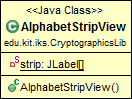
\includegraphics{resources/edu-kit-iks-CryptographicsLib-AlphabetStripView}
      \end{figure}
	
      \textbf{Superklassen und Interfaces}
      \begin{itemize}
        \item javax.swing.JPanel
      \end{itemize}
	
      \textbf{Methoden}
      \begin{itemize}
        \item public AlphabetStripView() \newline
          Konstruktor, der die Alphabetanzeige initialisiert.
      \end{itemize}
      
      \textbf{Getter}
      \begin{itemize}
		\item \textit{keine}
      \end{itemize}
      
      \textbf{Setter}
      \begin{itemize}
        \item \textit{keine}
      \end{itemize}
	% /AlphabetStripView
	
	% CustomButton
	\subsubsection{Klasse CustomButton}
	  todo
	
      \begin{figure}[H]
        \centering
        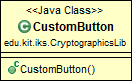
\includegraphics{resources/edu-kit-iks-CryptographicsLib-CustomButton}
      \end{figure}
	
      \textbf{Superklassen und Interfaces}
      \begin{itemize}
        \item \textit{keine}
      \end{itemize}
	
      \textbf{Methoden}
      \begin{itemize}
        \item public todo() \newline
          todo.
      \end{itemize}
      
      \textbf{Getter}
      \begin{itemize}
		\item \textit{keine}
      \end{itemize}
      
      \textbf{Setter}
      \begin{itemize}
        \item \textit{keine}
      \end{itemize}
	% /CustomButton	
	
	% CharacterFrequencyDiagramView
	\subsubsection{Klasse CharacterFrequencyDiagramView}
	  Instanzen dieser Klasse erzeugen ein Säulendiagramm, wobei die
	  Höhe jeder Säule die relative Häufigkeit eines Buchstaben in einem Text anzeigt.
	  Eine konkrete Instanz dieser Klasse kann aufgrund ihrer Vaterklasse als JPanel behandelt werden.
	
      \begin{figure}[H]
        \centering
        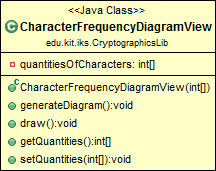
\includegraphics{resources/edu-kit-iks-CryptographicsLib-CharacterFrequencyDiagramView}
      \end{figure}
	
      \textbf{Superklassen und Interfaces}
      \begin{itemize}
        \item javax.swing.JPanel
      \end{itemize}
	
      \textbf{Methoden}
      \begin{itemize}
        \item public CharacterFrequencyDiagramView(int[] quantities) \newline
          Konstruktor, der mit den Häufigkeiten der einzelnen Buchstaben in einem Text
          initialisiert wird.
        \item public void generateDiagram() \newline
          Generiert das Diagramm anhand der gesetzten Parameter.
        \item public void drawDiagram() \newline
          Zeichnet das Diagramm.
      \end{itemize}
      
      \textbf{Getter}
      \begin{itemize}
		\item public int[] getQuantities()
      \end{itemize}
      
      \textbf{Setter}
      \begin{itemize}
        \item public void setQuantities(int[] quantitiesOfCharacters)
      \end{itemize}
	% /CharacterFrequencyDiagramView
	
	% ImageView
	\subsubsection{Klasse ImageView}
	  Instanzen dieser Klasse erzeugen ein JPanel, das ein Bild darstellt, welches
	  durch überschriebene Konstruktoren auf verschiedene Weisen initialisiert werden kann. 
	
      \begin{figure}[H]
        \centering
        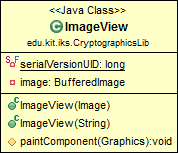
\includegraphics{resources/edu-kit-iks-CryptographicsLib-ImageView}
      \end{figure}
	
      \textbf{Superklassen und Interfaces}
      \begin{itemize}
        \item javax.swing.JPanel
      \end{itemize}
	
      \textbf{Methoden}
      \begin{itemize}
        \item public ImageView(Image img) \newline
          Konstruktor, der die Instanz anhand eines Image-Objekts initialisiert.
        \item public ImageView(String filePath) \newline
          Konstruktor, der die Instanz anhand eines Bilddateipfads initialisiert.
        \item protected void paintComponent(Graphics g) \newline
          Überschreibt javax.swing.JComponent\#paintComponent(java.awt.Graphics)
      \end{itemize}
      
      \textbf{Getter}
      \begin{itemize}
		\item \textit{keine}
      \end{itemize}
      
      \textbf{Setter}
      \begin{itemize}
        \item \textit{keine}
      \end{itemize}
	% /ImageView	
	
	% InformationController
	\subsubsection{Klasse InformationController}
	  Der InformationController ist ein von den Verfahren gemeinsam genutzter
	  Controller um weiterführende Informationen anzuzeigen, wobei dieser Controller
	  die für das Verfahren notwendige Informationsseite anhand der übergebenen VisualizationInfo
	  selbst initialisiert.
	
      \begin{figure}[H]
        \centering
        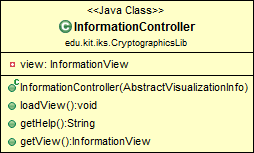
\includegraphics{resources/edu-kit-iks-CryptographicsLib-InformationController}
      \end{figure}
	
      \textbf{Superklassen und Interfaces}
      \begin{itemize}
        \item edu.kit.iks.CryptographicsLib.AbstractVisualizationController
      \end{itemize}
	
      \textbf{Methoden}
      \begin{itemize}
        \item public InformationController(AbstractVisualizationInfo visualizationInfo) \newline
          Konstruktor, der die Informationsseite anhand der übergebenen VisualizationInfo
          selbstständig initialisiert.
		\item public void loadView() \newline
		  Überschreibt edu.kit.iks.CryptographicsLib.AbstractController\#loadView()
		\item public String getHelp() \newline
		  Überschreibt edu.kit.iks.CryptographicsLib.AbstractVisualizationController\#getHelp()
		\item public InformationView getView() \newline
		  Überschreibt edu.kit.iks.CryptographicsLib.AbstractController\#getView()
      \end{itemize}
      
      \textbf{Getter}
      \begin{itemize}
		\item \textit{keine}
      \end{itemize}
      
      \textbf{Setter}
      \begin{itemize}
        \item \textit{keine}
      \end{itemize}
	% /InformationController	
	
	% InformationView
	\subsubsection{Klasse InformationView}
	  Instanzen dieser Klasse stellen eine View für den InformationController dar.
	  Zur Initialisierung benötigt diese Klasse das QR-Code-Bild zu den weiterführenden 
	  Informationen, sowie den Pfad zur lokalen HTML-Datei mit Informationen zum
	  aktuellen Verfahren.
	
      \begin{figure}[H]
        \centering
        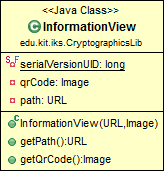
\includegraphics{resources/edu-kit-iks-CryptographicsLib-InformationView}
      \end{figure}
	
      \textbf{Superklassen und Interfaces}
      \begin{itemize}
        \item javax.swing.JPanel
      \end{itemize}
	
      \textbf{Methoden}
      \begin{itemize}
        \item public InformationView(URL path, Image qrCode) \newline
          Konstruktor, der die View mit dem QR-Code-Bild und der lokalen HTML-Datei füllt.
      \end{itemize}
      
      \textbf{Getter}
      \begin{itemize}
		\item public URL getPath()
		\item public Image getQrCode()
      \end{itemize}
      
      \textbf{Setter}
      \begin{itemize}
        \item \textit{keine}
      \end{itemize}
	% /InformationView	
	
	% KeyboardButton
	\subsubsection{Klasse KeyboardButton}
	  todo
	
      \begin{figure}[H]
        \centering
        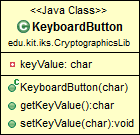
\includegraphics{resources/edu-kit-iks-CryptographicsLib-KeyboardButton}
      \end{figure}
	
      \textbf{Superklassen und Interfaces}
      \begin{itemize}
        \item \textit{keine}
      \end{itemize}
	
      \textbf{Methoden}
      \begin{itemize}
        \item public todo() \newline
          todo.
      \end{itemize}
      
      \textbf{Getter}
      \begin{itemize}
		\item \textit{keine}
      \end{itemize}
      
      \textbf{Setter}
      \begin{itemize}
        \item \textit{keine}
      \end{itemize}
	% /KeyboardButton	
	
	% KeyboardView
	\subsubsection{Klasse KeyboardView}
	  todo
	
      \begin{figure}[H]
        \centering
        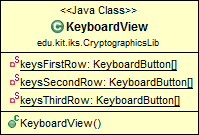
\includegraphics{resources/edu-kit-iks-CryptographicsLib-KeyboardView}
      \end{figure}
	
      \textbf{Superklassen und Interfaces}
      \begin{itemize}
        \item \textit{keine}
      \end{itemize}
	
      \textbf{Methoden}
      \begin{itemize}
        \item public todo() \newline
          todo.
      \end{itemize}
      
      \textbf{Getter}
      \begin{itemize}
		\item \textit{keine}
      \end{itemize}
      
      \textbf{Setter}
      \begin{itemize}
        \item \textit{keine}
      \end{itemize}
	% /KeyboardView	
	
	% NumbersStripView
	\subsubsection{Klasse NumbersStripView}
	  todo
	
      \begin{figure}[H]
        \centering
        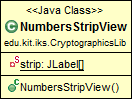
\includegraphics{resources/edu-kit-iks-CryptographicsLib-NumbersStripView}
      \end{figure}
	
      \textbf{Superklassen und Interfaces}
      \begin{itemize}
        \item \textit{keine}
      \end{itemize}
	
      \textbf{Methoden}
      \begin{itemize}
        \item public todo() \newline
          todo.
      \end{itemize}
      
      \textbf{Getter}
      \begin{itemize}
		\item \textit{keine}
      \end{itemize}
      
      \textbf{Setter}
      \begin{itemize}
        \item \textit{keine}
      \end{itemize}
	% /NumbersStripView	
	
	% PopoverView
	\subsubsection{Klasse PopoverView}
	  Diese Klasse ist als Oberklasse für konkrete Popover gedacht. Sie
	  bündelt die Funktionalitäten, die jeder Popover des Programms haben muss.
	
      \begin{figure}[H]
        \centering
        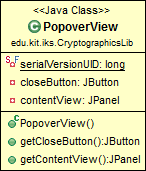
\includegraphics{resources/edu-kit-iks-CryptographicsLib-PopoverView}
      \end{figure}
	
      \textbf{Superklassen und Interfaces}
      \begin{itemize}
        \item javax.swing.JPanel
      \end{itemize}
	
      \textbf{Methoden}
      \begin{itemize}
        \item public PopoverView() \newline
          Konstruktor, der ein Popover erzeugt und alle gemeinsamen Komponenten wie
          die Buttons initialisiert.
      \end{itemize}
      
      \textbf{Getter}
      \begin{itemize}
		\item public JButton getCloseButton()
		\item public JPanel getContentView()
      \end{itemize}
      
      \textbf{Setter}
      \begin{itemize}
        \item \textit{keine}
      \end{itemize}
	% /PopoverView	
	
	% VisualizationButton
	\subsubsection{Klasse VisualizationButton}
	  todo
	
      \begin{figure}[H]
        \centering
        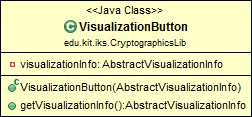
\includegraphics{resources/edu-kit-iks-CryptographicsLib-VisualizationButton}
      \end{figure}
	
      \textbf{Superklassen und Interfaces}
      \begin{itemize}
        \item \textit{keine}
      \end{itemize}
	
      \textbf{Methoden}
      \begin{itemize}
        \item public todo() \newline
          todo.
      \end{itemize}
      
      \textbf{Getter}
      \begin{itemize}
		\item \textit{keine}
      \end{itemize}
      
      \textbf{Setter}
      \begin{itemize}
        \item \textit{keine}
      \end{itemize}
	% /VisualizationButton	
	
	% VisualizationDifficulty
	\subsubsection{Enum VisualizationDifficulty}
	  todo
	
      \begin{figure}[H]
        \centering
        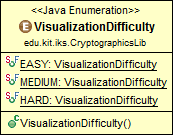
\includegraphics{resources/edu-kit-iks-CryptographicsLib-VisualizationDifficulty}
      \end{figure}

      \textbf{Werte}
      \begin{itemize}
        \item EASY \newline
          Schwierigkeitsgrad \glqq Einfach\grqq.
        \item MEDIUM \newline
          Schwierigkeitsgrad \glqq Mittel\grqq.
        \item HARD \newline
          Schwierigkeitsgrad \glqq Schwer\grqq.
      \end{itemize}
	% /VisualizationDifficulty	
	
	% VisualizationInfoLoader
	\subsubsection{Klasse VisualizationInfoLoader}
	  Diese Klasse bietet mit ihrer einzigen statischen Methode eine Möglichkeit, 
	  die VisualizationInfos sämtlicher Verfahren zu beziehen.
	
      \begin{figure}[H]
        \centering
        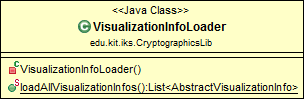
\includegraphics{resources/edu-kit-iks-CryptographicsLib-VisualizationInfoLoader}
      \end{figure}
	
      \textbf{Superklassen und Interfaces}
      \begin{itemize}
        \item \textit{keine}
      \end{itemize}
	
      \textbf{Methoden}
      \begin{itemize}
        \item static public List<AbstractVisualizationInfo> loadAllVisualizationInfos() \newline
          Bezieht eine Liste der VisualizationInfos sämtlicher Verfahren.
      \end{itemize}
      
      \textbf{Getter}
      \begin{itemize}
		\item \textit{keine}
      \end{itemize}
      
      \textbf{Setter}
      \begin{itemize}
        \item \textit{keine}
      \end{itemize}
	% /VisualizationInfoLoader	
	
	% VisualizationView
	\subsubsection{Klasse VisualizationView}
	  Die VisualizationView vereint gemeinsame Komponenten, die die Visualisierungen
	  untereinander teilen.
	
      \begin{figure}[H]
        \centering
        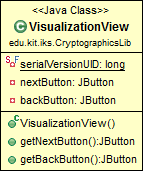
\includegraphics{resources/edu-kit-iks-CryptographicsLib-VisualizationView}
      \end{figure}
	
      \textbf{Superklassen und Interfaces}
      \begin{itemize}
        \item javax.swing.JPanel
      \end{itemize}
	
      \textbf{Methoden}
      \begin{itemize}
        \item public VisualizationView() \newline
          Konstruktor, der die gemeinsamen Komponenten initialisiert.
      \end{itemize}
      
      \textbf{Getter}
      \begin{itemize}
		\item public JButton getNextButton()
		\item public JButton getBackButton()
      \end{itemize}
      
      \textbf{Setter}
      \begin{itemize}
        \item \textit{keine}
      \end{itemize}
	% /VisualizationView	
	
  \subsection{Paket edu.kit.iks.Cryptographics.Vigenere}
    \subsubsection{Klasse AbstractController}
      Der AbstractController ist eine abstrakte Klasse, die die verschiedenen State-Controller im Vigenere-Paket nutzen.
      \begin{figure}[H]
        \centering
        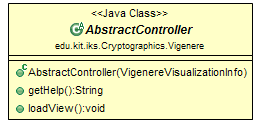
\includegraphics{resources/edu-kit-iks-Cryptographics-Vigenere-AbstractController}
      \end{figure}

      \textbf{Superklassen und Interfaces}
      \begin{itemize}
        \item edu.kit.iks.CryptographicsLib.AbstractVisualizationController
      \end{itemize}
      
      \textbf{Methoden}
      \begin{itemize}
        \item public String getHelp() \newline
        Gibt den Hilfe-Text an.
        \item public String loadView() \newline
        Lädt die View zum zugehörigen Zustand.
      \end{itemize}

    \subsubsection{Klasse VigenereModel}
      Das VigenereModel ist für die Ver- und Entschlüsselung zuständig.
      \begin{figure}[H]
        \centering
        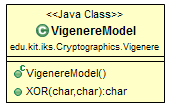
\includegraphics{resources/edu-kit-iks-Cryptographics-Vigenere-VigenereModel}
      \end{figure}
      
      \textbf{Methoden}
      \begin{itemize}
        \item public char XOR(char a, char b) \newline
        Benutzt einen logischen XOR auf die Parameter a und b.
      \end{itemize}

    \subsubsection{Klasse VigenereVisualizationInfo}
      VigenereVisualizationInfo enthält alle wichtigen Informationen zu dem Verfahren, wie z.B. Verfahrensname/Beschreibung.
      \begin{figure}[H]
        \centering
        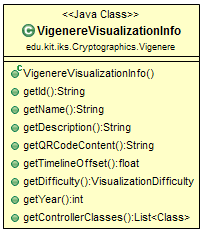
\includegraphics{resources/edu-kit-iks-Cryptographics-Vigenere-VisualizationInfo}
      \end{figure}

      \textbf{Superklassen und Interfaces}
      \begin{itemize}
        \item edu.kit.iks.CryptographicsLib.AbstractVisualizationInfo
      \end{itemize}
      
      \textbf{Methoden}
      \begin{itemize}
        \item public String getId() \newline
        Gibt die Kennungs-ID aus.
        \item public String getName() \newline
        Gibt den Namen des Verfahrens aus.
        \item public String getDescription() \newline
        Gibt die Beschreibung des Verfahrens aus.
        \item public String getQRCodeContent() \newline
        Gibt den Inhalt des QRCodes aus.
        \item public float getTimelineOffset() \newline
        Gibt die relative Position in der Timeline aus.
        \item public VisualizationDifficulty getDifficulty() \newline
        Gibt den Schwierigkeitsgrad aus.
        \item public int getYear() \newline
        Gibt das Jahr aus, in welchem das Verfahren entwickelt wurde.
        \item public List<Class> getControllerClasses() \newline
        Gibt eine Liste von Controller-Klassen des Verfahrens aus, welche dann im Statecontroller geswitcht werden können.
      \end{itemize}

  \subsection{Paket edu.kit.iks.Cryptographics.Vigenere.Demonstration}
    \subsubsection{Klasse FirstDemonstrationController}
      Der FirstDemonstrationController erstellt FirstDemonstrationView.
      \begin{figure}[H]
        \centering
        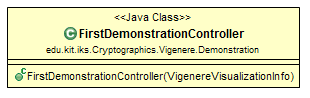
\includegraphics{resources/edu-kit-iks-Cryptographics-Vigenere-FirstDemonstrationController}
      \end{figure}

      \textbf{Superklassen und Interfaces}
      \begin{itemize}
        \item edu.kit.iks.CryptographicsLib.AbstractController
      \end{itemize}

    \subsubsection{Klasse FirstDemonstrationView}
      Die FirstDemonstrationView zeigt die Informationen über Vigenere sowie eine kurze Erklärung über Modulo.
      \begin{figure}[H]
        \centering
        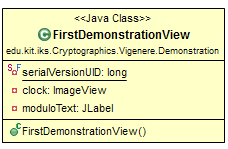
\includegraphics{resources/edu-kit-iks-Cryptographics-Vigenere-FirstDemonstrationView}
      \end{figure}

      \textbf{Superklassen und Interfaces}
      \begin{itemize}
        \item edu.kit.iks.CryptographicsLib.VisualizationView
      \end{itemize}

    \subsubsection{Klasse SecondDemonstrationController}
      Der SecondDemonstrationController erstellt SecondDemonstrationView.
      \begin{figure}[H]
        \centering
        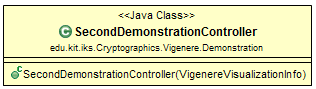
\includegraphics{resources/edu-kit-iks-Cryptographics-Vigenere-SecondDemonstrationController}
      \end{figure}

      \textbf{Superklassen und Interfaces}
      \begin{itemize}
        \item edu.kit.iks.CryptographicsLib.AbstractController
      \end{itemize}

    \subsubsection{Klasse SecondDemonstrationView}
      Die SecondDemonstrationView zeigt eine Animation über die Funktionsweise der Verschlüsselung mit Vigenere.
      \begin{figure}[H]
        \centering
        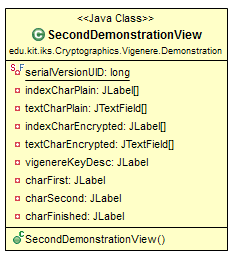
\includegraphics{resources/edu-kit-iks-Cryptographics-Vigenere-SecondDemonstrationView}
      \end{figure}

      \textbf{Superklassen und Interfaces}
      \begin{itemize}
        \item edu.kit.iks.CryptographicsLib.VisualizationView
      \end{itemize}

    \subsubsection{Klasse ThirdDemonstrationController}
      Der ThirdDemonstrationController erstellt ThirdDemonstrationView.
      \begin{figure}[H]
        \centering
        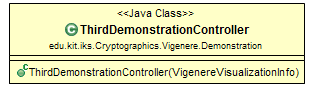
\includegraphics{resources/edu-kit-iks-Cryptographics-Vigenere-ThirdDemonstrationController}
      \end{figure}

      \textbf{Superklassen und Interfaces}
      \begin{itemize}
        \item edu.kit.iks.CryptographicsLib.AbstractController
      \end{itemize}

    \subsubsection{Klasse ThirdDemonstrationView}
      Die ThirdDemonstrationView zeigt eine Animation über die Funktionsweise der Entschlüsselung mit Vigenere.
      \begin{figure}[H]
        \centering
        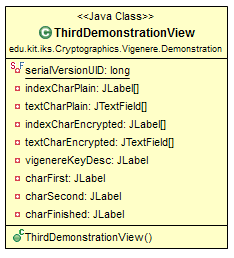
\includegraphics{resources/edu-kit-iks-Cryptographics-Vigenere-ThirdDemonstrationView}
      \end{figure}

      \textbf{Superklassen und Interfaces}
      \begin{itemize}
        \item edu.kit.iks.CryptographicsLib.VisualizationView
      \end{itemize}

  \subsection{Paket edu.kit.iks.Cryptographics.Vigenere.Experiment}
    \subsubsection{Klasse FirstExperimentController}
      Der FirstExperimentController erstellt FirstExperimentView.
      \begin{figure}[H]
        \centering
        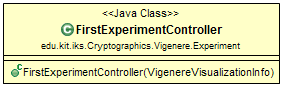
\includegraphics{resources/edu-kit-iks-Cryptographics-Vigenere-FirstExperimentController}
      \end{figure}

      \textbf{Superklassen und Interfaces}
      \begin{itemize}
        \item edu.kit.iks.CryptographicsLib.AbstractController
      \end{itemize}

    \subsubsection{Klasse FirstExperimentView}
      Die FirstExperimentView zeigt den Selbstversuch wobei der Nutzer einen selbst gewählten Text mit einem selbstgewähltem Passwort verschlüsseln muss und dieser hinterher von Cryptographics entschlüsselt wird.
      \begin{figure}[H]
        \centering
        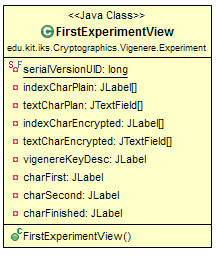
\includegraphics{resources/edu-kit-iks-Cryptographics-Vigenere-FirstExperimentView}
      \end{figure}

      \textbf{Superklassen und Interfaces}
      \begin{itemize}
        \item edu.kit.iks.CryptographicsLib.VisualizationView
      \end{itemize}

    \subsubsection{Klasse SecondExperimentController}
      Der SecondExperimentController erstellt SecondExperimentView.
      \begin{figure}[H]
        \centering
        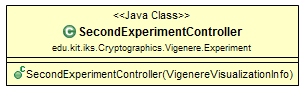
\includegraphics{resources/edu-kit-iks-Cryptographics-Vigenere-SecondExperimentController}
      \end{figure}

      \textbf{Superklassen und Interfaces}
      \begin{itemize}
        \item edu.kit.iks.CryptographicsLib.AbstractController
      \end{itemize}

    \subsubsection{Klasse SecondExperimentView}
      Die SecondExperimentView zeigt den Selbstversuch wobei der Nutzer einen generierten Text mit einem generierten Passwort entschlüsseln muss.
      \begin{figure}[H]
        \centering
        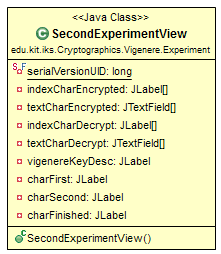
\includegraphics{resources/edu-kit-iks-Cryptographics-Vigenere-SecondExperimentView}
      \end{figure}

      \textbf{Superklassen und Interfaces}
      \begin{itemize}
        \item edu.kit.iks.CryptographicsLib.VisualizationView
      \end{itemize}

  \subsection{Paket edu.kit.iks.Cryptographics.Vigenere.Explanatation}
    \subsubsection{Klasse FirstExplanatationController}
      Der FirstExplanatationController erstellt FirstExplanatationView.
      \begin{figure}[H]
        \centering
        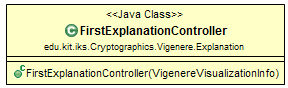
\includegraphics{resources/edu-kit-iks-Cryptographics-Vigenere-FirstExplanationController}
      \end{figure}

      \textbf{Superklassen und Interfaces}
      \begin{itemize}
        \item edu.kit.iks.CryptographicsLib.AbstractController
      \end{itemize}

    \subsubsection{Klasse FirstExplanatationView}
      Die FirstExperimentView zeigt die Schwachstellen und möglich Angriffspunkte von Vigenere.
      \begin{figure}[H]
        \centering
        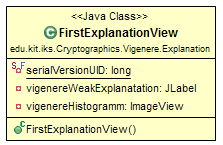
\includegraphics{resources/edu-kit-iks-Cryptographics-Vigenere-FirstExplanationView}
      \end{figure}

      \textbf{Superklassen und Interfaces}
      \begin{itemize}
        \item edu.kit.iks.CryptographicsLib.VisualizationView
      \end{itemize}

    \subsubsection{Klasse SecondExplanatationController}
      Der SecondExplanatationController erstellt SecondExplanatationView.
      \begin{figure}[H]
        \centering
        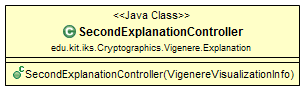
\includegraphics{resources/edu-kit-iks-Cryptographics-Vigenere-SecondExplanationController}
      \end{figure}

      \textbf{Superklassen und Interfaces}
      \begin{itemize}
        \item edu.kit.iks.CryptographicsLib.AbstractController
      \end{itemize}

    \subsubsection{Klasse SecondExplanatationView}
      Die SecondExplanatationView zeigt den Selbstversuch wobei der Nutzer ein Histogramm generieren, die Schlüssellänge berechnen lassen kann und dann den Key finden muss.
      \begin{figure}[H]
        \centering
        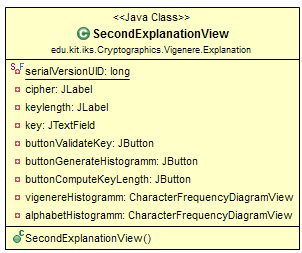
\includegraphics{resources/edu-kit-iks-Cryptographics-Vigenere-SecondExplanationView}
      \end{figure}

      \textbf{Superklassen und Interfaces}
      \begin{itemize}
        \item edu.kit.iks.CryptographicsLib.VisualizationView
      \end{itemize}

\subsection{Paket edu.kit.iks.Cryptographics.Caesar}

\subsection{Paket edu.kit.iks.Cryptographics.DiffieHellman}
\subsubsection{Klasse Model}
      Das Model in MVC für die Diffie-Hellman Analogie.
      Diese Klasse verwendet das Singleton Entwurfsmuster,
      da die unterschiedliche Controller das gleiche Model sollen.

      \begin{figure}[H]
        \centering
        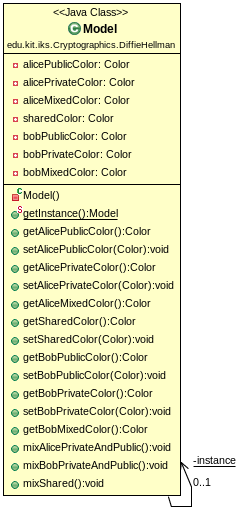
\includegraphics{resources/edu-kit-iks-Cryptographics-DiffieHellman-Model}
      \end{figure}

      \textbf{Superklassen und Interfaces}
      \begin{itemize}
        \item \textit{keine}
      \end{itemize}

      \textbf{Methoden}
      \begin{itemize}
        \item public static Model getInstance() \newline
            Fabrikmethode um das Singleton-Muster zu implementieren.
            Verwendet Lazy-Evaluation.
        \item public void mixAlicePrivateAndPublic() \newline
            Mische die private und öffentliche Farbe
            von Alice. Entspricht der modularen Exponentiation
            im echten Diffie-Hellman verfahren.
        \item public void mixBobPrivateAndPublic() \newline
            Mische die private und öffentliche Farbe
            von Bob. Entspricht der modularen Exponentiation
            im echten Diffie-Hellman verfahren.
        \item public void mixShared() \newline
            Mische die jeweiligen private Farben
            zu den bereits gemischten Farben
            um das gemeinsame Geheimnis zu erhalten.
      \end{itemize}

      \textbf{Getter}
      \begin{itemize}
        \item public Color getAlicPublicColor()
        \item public Color getAlicePrivateColor()
        \item public Color getAliceMixedColor()
        \item public Color getSharedColor()
        \item public Color getBobPublicColor
        \item public Color getBobPrivateColor()
        \item public Color getBobMixedColor()
      \end{itemize}

      \textbf{Setter}
      \begin{itemize}
        \item public void setAlicPublicColor(Color alicePublicColor)
        \item public void setAlicePrivateColor(Color alicePrivateColor)
        \item public void setSharedColor(Color sharedColor)
        \item public void setBobPublicColor(Color bobPublicColor)
      \end{itemize}

\subsubsection{Klasse DHVisualizationInfo}
      DHVisualizationInfo enthält alle wichtigen Informationen zu dem Verfahren, wie z.B. Verfahrensname/Beschreibung.
      \begin{figure}[H]
        \centering
        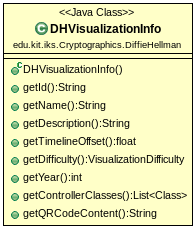
\includegraphics{resources/edu-kit-iks-Cryptographics-DiffieHellman-DHVisualizationInfo}
      \end{figure}

      \textbf{Superklassen und Interfaces}
      \begin{itemize}
        \item edu.kit.iks.CryptographicsLib.AbstractVisualizationInfo
      \end{itemize}
      
      \textbf{Methoden}
      \begin{itemize}
        \item public String getId() \newline
        Gibt die Kennungs-ID aus.
        \item public String getName() \newline
        Gibt den Namen des Verfahrens aus.
        \item public String getDescription() \newline
        Gibt die Beschreibung des Verfahrens aus.
        \item public String getQRCodeContent() \newline
        Gibt den Inhalt des QRCodes aus.
        \item public float getTimelineOffset() \newline
        Gibt die relative Position in der Timeline aus.
        \item public VisualizationDifficulty getDifficulty() \newline
        Gibt den Schwierigkeitsgrad aus.
        \item public int getYear() \newline
        Gibt das Jahr aus, in welchem das Verfahren entwickelt wurde.
        \item public List<Class> getControllerClasses() \newline
        Gibt eine Liste von Controller-Klassen des Verfahrens aus, welche dann im Statecontroller geswitcht werden können.
      \end{itemize}

\subsection{Paket edu.kit.iks.Cryptographics.DiffieHellman.Demonstration}

\subsubsection{Klasse ExplainAimController}
      Der erste StateController für die Demonstration der Diffie-Hellman Analogie.
      Der ExplainAim Zustand, erklärt was wir eigentlich erreichen wollen,
      nämlich ein gemeinsames Geheimnis auf einem unsicheren Kanal austauschen.
      Verwendet das Diffie-Hellman Model und die ExplainAimView.

      \begin{figure}[H]
        \centering
        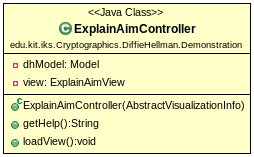
\includegraphics[width=\textwidth]{resources/edu-kit-iks-Cryptographics-DiffieHellman-Demonstration-ExplainAimController}
      \end{figure}

      \textbf{Superklassen und Interfaces}
      \begin{itemize}
        \item edu.kit.iks.CryptographicsLib.AbstractVisualizationController
      \end{itemize}

      \textbf{Methoden}
      \begin{itemize}
          \item public ExplainAimController(AbstractVisualizationInfo visualizationInfo) \newline
              Holt sich sein DiffieHellman Model Singleton und instanziiert seine View
        \item public String getHelp() \newline
        Gibt den Hilfe-Text an.
        \item public String loadView() \newline
        Lädt die View zum zugehörigen Zustand.
      \end{itemize}

\subsubsection{Klasse ExplainAimView}
      Die erste StateView für die Demonstration der Diffie-Hellman Analogie.
      Der ExplainAim Zustand, erklärt was wir eigentlich erreichen wollen,
      nämlich ein gemeinsames Geheimnis auf einem unsicheren Kanal austauschen.

      \begin{figure}[H]
        \centering
        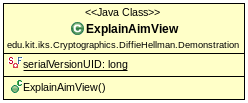
\includegraphics[width=\textwidth]{resources/edu-kit-iks-Cryptographics-DiffieHellman-Demonstration-ExplainAimView}
      \end{figure}

      \textbf{Superklassen und Interfaces}
      \begin{itemize}
        \item edu.kit.iks.CryptographicsLib.VisualizationView
      \end{itemize}

      \textbf{Methoden}
      \begin{itemize}
        \item \textit{keine}
      \end{itemize}

\subsubsection{Klasse OnewayController}
      Der zweite StateController für die Demonstration der Diffie-Hellman Analogie.
      Der OnewayController Zustand, erklärt wie wir dies durch Einwegfunktionen
      erreichen können. Dazu erklärt er an einer Analogie das Konzept
      der Einwegfunktion.
      Verwendet das Diffie-Hellman Model und die OnewayView.

      \begin{figure}[H]
        \centering
        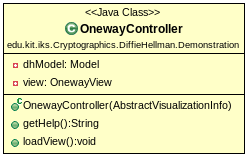
\includegraphics[width=\textwidth]{resources/edu-kit-iks-Cryptographics-DiffieHellman-Demonstration-OnewayController}
      \end{figure}

      \textbf{Superklassen und Interfaces}
      \begin{itemize}
        \item edu.kit.iks.CryptographicsLib.AbstractVisualizationController
      \end{itemize}

      \textbf{Methoden}
      \begin{itemize}
          \item public OnewayController(AbstractVisualizationInfo visualizationInfo) \newline
              Holt sich sein DiffieHellman Model Singleton und instanziiert seine View
        \item public String getHelp() \newline
        Gibt den Hilfe-Text an.
        \item public String loadView() \newline
        Lädt die View zum zugehörigen Zustand.
      \end{itemize}

\subsubsection{Klasse OnewayView}
      Die zweite StateView für die Demonstration der Diffie-Hellman Analogie.
      Der Oneway Zustand, erklärt was wir eigentlich erreichen wollen,
      nämlich ein gemeinsames Geheimnis auf einem unsicheren Kanal austauschen.

      \begin{figure}[H]
        \centering
        \includegraphics[width=\textwidth]{resources/edu-kit-iks-Cryptographics-DiffieHellman-Demonstration-OnewayView}
      \end{figure}

      \textbf{Superklassen und Interfaces}
      \begin{itemize}
        \item edu.kit.iks.CryptographicsLib.VisualizationView
      \end{itemize}

      \textbf{Methoden}
      \begin{itemize}
        \item \textit{keine}
      \end{itemize}

\subsubsection{Klasse ExplainKeyExchangeController}
      Der dritte StateController für die Demonstration der Diffie-Hellman Analogie.
      Verwendet das Diffie-Hellman Model und die ExplainKeyExchangeView.

      \begin{figure}[H]
        \centering
        \includegraphics[width=\textwidth]{resources/edu-kit-iks-Cryptographics-DiffieHellman-Demonstration-ExplainKeyExchangeController}
      \end{figure}

      \textbf{Superklassen und Interfaces}
      \begin{itemize}
        \item edu.kit.iks.CryptographicsLib.AbstractVisualizationController
      \end{itemize}

      \textbf{Methoden}
      \begin{itemize}
          \item public ExplainKeyExchangeController(AbstractVisualizationInfo visualizationInfo) \newline
              Holt sich sein DiffieHellman Model Singleton und instanziert seine View
        \item public String getHelp() \newline
        Gibt den Hilfe-Text an.
        \item public String loadView() \newline
        Lädt die View zum zugehörigen Zustand.
      \end{itemize}

\subsubsection{Klasse ExplainKeyExchangeView}
      Die erste StateView für die Demonstration der Diffie-Hellman Analogie.
      Der ExplainKeyExchange Zustand, erklärt was wir eigentlich erreichen wollen,
      nämlich ein gemeinsames Geheimnis auf einem unsicheren Kanal austauschen.

      \begin{figure}[H]
        \centering
        \includegraphics[width=\textwidth]{resources/edu-kit-iks-Cryptographics-DiffieHellman-Demonstration-ExplainKeyExchangeView}
      \end{figure}

      \textbf{Superklassen und Interfaces}
      \begin{itemize}
        \item edu.kit.iks.CryptographicsLib.VisualizationView
      \end{itemize}

      \textbf{Methoden}
      \begin{itemize}
        \item \textit{keine}
      \end{itemize}

\subsubsection{Klasse AliceChooseSecretController}
      Der vierte StateController für die Demonstration der Diffie-Hellman Analogie.
      Verwendet das Diffie-Hellman Model und die AliceChooseSecretView.

      \begin{figure}[H]
        \centering
        \includegraphics[width=\textwidth]{resources/edu-kit-iks-Cryptographics-DiffieHellman-Demonstration-AliceChooseSecretController}
      \end{figure}

      \textbf{Superklassen und Interfaces}
      \begin{itemize}
        \item edu.kit.iks.CryptographicsLib.AbstractVisualizationController
      \end{itemize}

      \textbf{Methoden}
      \begin{itemize}
          \item public AliceChooseSecretController(AbstractVisualizationInfo visualizationInfo) \newline
              Holt sich sein DiffieHellman Model Singleton und instanziert seine View
        \item public String getHelp() \newline
        Gibt den Hilfe-Text an.
        \item public String loadView() \newline
        Lädt die View zum zugehörigen Zustand.
      \end{itemize}

\subsubsection{Klasse AliceChooseSecretView}
      Die vierte StateView für die Demonstration der Diffie-Hellman Analogie.
      Der AliceChooseSecret Zustand, erklärt was wir eigentlich erreichen wollen,
      nämlich ein gemeinsames Geheimnis auf einem unsicheren Kanal austauschen.

      \begin{figure}[H]
        \centering
        \includegraphics[width=\textwidth]{resources/edu-kit-iks-Cryptographics-DiffieHellman-Demonstration-AliceChooseSecretView}
      \end{figure}

      \textbf{Superklassen und Interfaces}
      \begin{itemize}
        \item edu.kit.iks.CryptographicsLib.VisualizationView
      \end{itemize}

      \textbf{Methoden}
      \begin{itemize}
        \item \textit{keine}
      \end{itemize}

\subsubsection{Klasse BobChooseSecretController}
      Der fünfte StateController für die Demonstration der Diffie-Hellman Analogie.
      Verwendet das Diffie-Hellman Model und die BobChooseSecretView.

      \begin{figure}[H]
        \centering
        \includegraphics[width=\textwidth]{resources/edu-kit-iks-Cryptographics-DiffieHellman-Demonstration-BobChooseSecretController}
      \end{figure}

      \textbf{Superklassen und Interfaces}
      \begin{itemize}
        \item edu.kit.iks.CryptographicsLib.AbstractVisualizationController
      \end{itemize}

      \textbf{Methoden}
      \begin{itemize}
          \item public BobChooseSecretController(AbstractVisualizationInfo visualizationInfo) \newline
              Holt sich sein DiffieHellman Model Singleton und instanziert seine View
        \item public String getHelp() \newline
        Gibt den Hilfe-Text an.
        \item public String loadView() \newline
        Lädt die View zum zugehörigen Zustand.
      \end{itemize}

\subsubsection{Klasse BobChooseSecretView}
      Die fünfte StateView für die Demonstration der Diffie-Hellman Analogie.
      Der BobChooseSecret Zustand, erklärt was wir eigentlich erreichen wollen,
      nämlich ein gemeinsames Geheimnis auf einem unsicheren Kanal austauschen.

      \begin{figure}[H]
        \centering
        \includegraphics[width=\textwidth]{resources/edu-kit-iks-Cryptographics-DiffieHellman-Demonstration-BobChooseSecretView}
      \end{figure}

      \textbf{Superklassen und Interfaces}
      \begin{itemize}
        \item edu.kit.iks.CryptographicsLib.VisualizationView
      \end{itemize}

      \textbf{Methoden}
      \begin{itemize}
        \item \textit{keine}
      \end{itemize}

\subsubsection{Klasse MixColorController}
      Der sechste StateController für die Demonstration der Diffie-Hellman Analogie.
      Verwendet das Diffie-Hellman Model und die MixColorView.

      \begin{figure}[H]
        \centering
        \includegraphics[width=\textwidth]{resources/edu-kit-iks-Cryptographics-DiffieHellman-Demonstration-MixColorController}
      \end{figure}

      \textbf{Superklassen und Interfaces}
      \begin{itemize}
        \item edu.kit.iks.CryptographicsLib.AbstractVisualizationController
      \end{itemize}

      \textbf{Methoden}
      \begin{itemize}
          \item public MixColorController(AbstractVisualizationInfo visualizationInfo) \newline
              Holt sich sein DiffieHellman Model Singleton und instanziert seine View
        \item public String getHelp() \newline
        Gibt den Hilfe-Text an.
        \item public String loadView() \newline
        Lädt die View zum zugehörigen Zustand.
      \end{itemize}

\subsubsection{Klasse MixColorView}
      Die erste StateView für die Demonstration der Diffie-Hellman Analogie.
      Der MixColor Zustand, erklärt was wir eigentlich erreichen wollen,
      nämlich ein gemeinsames Geheimnis auf einem unsicheren Kanal austauschen.

      \begin{figure}[H]
        \centering
        \includegraphics[width=\textwidth]{resources/edu-kit-iks-Cryptographics-DiffieHellman-Demonstration-MixColorView}
      \end{figure}

      \textbf{Superklassen und Interfaces}
      \begin{itemize}
        \item edu.kit.iks.CryptographicsLib.VisualizationView
      \end{itemize}

      \textbf{Methoden}
      \begin{itemize}
        \item \textit{keine}
      \end{itemize}

\subsection{Paket edu.kit.iks.Cryptographics.DiffieHellman.Experiment}

\subsubsection{Klasse YourTurnController}
      Der erste StateController für das Experiment der Diffie-Hellman Analogie.
      Der YourTurn Zustand, erklärt was wir eigentlich erreichen wollen,
      nämlich ein gemeinsames Geheimnis auf einem unsicheren Kanal austauschen.
      Verwendet das Diffie-Hellman Model und die YourTurnView.

      \begin{figure}[H]
        \centering
        \includegraphics[width=\textwidth]{resources/edu-kit-iks-Cryptographics-DiffieHellman-Experiment-YourTurnController}
      \end{figure}

      \textbf{Superklassen und Interfaces}
      \begin{itemize}
        \item edu.kit.iks.CryptographicsLib.AbstractVisualizationController
      \end{itemize}

      \textbf{Methoden}
      \begin{itemize}
          \item public YourTurnController(AbstractVisualizationInfo visualizationInfo) \newline
              Holt sich sein DiffieHellman Model Singleton und instanziiert seine View
        \item public String getHelp() \newline
        Gibt den Hilfe-Text an.
        \item public String loadView() \newline
        Lädt die View zum zugehörigen Zustand.
      \end{itemize}

\subsubsection{Klasse YourTurnView}
      Der erste StateView für das Experiment der Diffie-Hellman Analogie.
      Der YourTurn Zustand, erklärt was wir eigentlich erreichen wollen,
      nämlich ein gemeinsames Geheimnis auf einem unsicheren Kanal austauschen.

      \begin{figure}[H]
        \centering
        \includegraphics[width=\textwidth]{resources/edu-kit-iks-Cryptographics-DiffieHellman-Experiment-YourTurnView}
      \end{figure}

      \textbf{Superklassen und Interfaces}
      \begin{itemize}
        \item javax.swing.JPanel
      \end{itemize}

      \textbf{Methoden}
      \begin{itemize}
        \item \textit{keine}
      \end{itemize}

\subsubsection{Klasse ChoosePublicColorController}
      Der erste StateController für das Experiment der Diffie-Hellman Analogie.
      Der ChoosePublicColor Zustand, erklärt was wir eigentlich erreichen wollen,
      nämlich ein gemeinsames Geheimnis auf einem unsicheren Kanal austauschen.
      Verwendet das Diffie-Hellman Model und die ChoosePublicColorView.

      \begin{figure}[H]
        \centering
        \includegraphics[width=\textwidth]{resources/edu-kit-iks-Cryptographics-DiffieHellman-Experiment-ChoosePublicColorController}
      \end{figure}

      \textbf{Superklassen und Interfaces}
      \begin{itemize}
        \item edu.kit.iks.CryptographicsLib.AbstractVisualizationController
      \end{itemize}

      \textbf{Methoden}
      \begin{itemize}
          \item public ChoosePublicColorController(AbstractVisualizationInfo visualizationInfo) \newline
              Holt sich sein DiffieHellman Model Singleton und instanziiert seine View
        \item public String getHelp() \newline
        Gibt den Hilfe-Text an.
        \item public String loadView() \newline
        Lädt die View zum zugehörigen Zustand.
      \end{itemize}

\subsubsection{Klasse ChoosePublicColorView}
      Der erste StateView für das Experiment der Diffie-Hellman Analogie.
      Der ChoosePublicColor Zustand, erklärt was wir eigentlich erreichen wollen,
      nämlich ein gemeinsames Geheimnis auf einem unsicheren Kanal austauschen.

      \begin{figure}[H]
        \centering
        \includegraphics[width=\textwidth]{resources/edu-kit-iks-Cryptographics-DiffieHellman-Experiment-ChoosePublicColorView}
      \end{figure}

      \textbf{Superklassen und Interfaces}
      \begin{itemize}
        \item javax.swing.JPanel
      \end{itemize}

      \textbf{Methoden}
      \begin{itemize}
        \item \textit{keine}
      \end{itemize}

\subsubsection{Klasse SendColorController}
      Der erste StateController für das Experiment der Diffie-Hellman Analogie.
      Der SendColor Zustand, erklärt was wir eigentlich erreichen wollen,
      nämlich ein gemeinsames Geheimnis auf einem unsicheren Kanal austauschen.
      Verwendet das Diffie-Hellman Model und die SendColorView.

      \begin{figure}[H]
        \centering
        \includegraphics[width=\textwidth]{resources/edu-kit-iks-Cryptographics-DiffieHellman-Experiment-SendColorController}
      \end{figure}

      \textbf{Superklassen und Interfaces}
      \begin{itemize}
        \item edu.kit.iks.CryptographicsLib.AbstractVisualizationController
      \end{itemize}

      \textbf{Methoden}
      \begin{itemize}
          \item public SendColorController(AbstractVisualizationInfo visualizationInfo) \newline
              Holt sich sein DiffieHellman Model Singleton und instanziiert seine View
        \item public String getHelp() \newline
        Gibt den Hilfe-Text an.
        \item public String loadView() \newline
        Lädt die View zum zugehörigen Zustand.
      \end{itemize}

\subsubsection{Klasse SendColorView}
      Der erste StateView für das Experiment der Diffie-Hellman Analogie.
      Der SendColor Zustand, erklärt was wir eigentlich erreichen wollen,
      nämlich ein gemeinsames Geheimnis auf einem unsicheren Kanal austauschen.

      \begin{figure}[H]
        \centering
        \includegraphics[width=\textwidth]{resources/edu-kit-iks-Cryptographics-DiffieHellman-Experiment-SendColorView}
      \end{figure}

      \textbf{Superklassen und Interfaces}
      \begin{itemize}
        \item javax.swing.JPanel
      \end{itemize}

      \textbf{Methoden}
      \begin{itemize}
        \item \textit{keine}
      \end{itemize}

\subsubsection{Klasse ChooseSecretColorController}
      Der erste StateController für das Experiment der Diffie-Hellman Analogie.
      Der ChooseSecretColor Zustand, erklärt was wir eigentlich erreichen wollen,
      nämlich ein gemeinsames Geheimnis auf einem unsicheren Kanal austauschen.
      Verwendet das Diffie-Hellman Model und die ChooseSecretColorView.

      \begin{figure}[H]
        \centering
        \includegraphics[width=\textwidth]{resources/edu-kit-iks-Cryptographics-DiffieHellman-Experiment-ChooseSecretColorController}
      \end{figure}

      \textbf{Superklassen und Interfaces}
      \begin{itemize}
        \item edu.kit.iks.CryptographicsLib.AbstractVisualizationController
      \end{itemize}

      \textbf{Methoden}
      \begin{itemize}
          \item public ChooseSecretColorController(AbstractVisualizationInfo visualizationInfo) \newline
              Holt sich sein DiffieHellman Model Singleton und instanziiert seine View
        \item public String getHelp() \newline
        Gibt den Hilfe-Text an.
        \item public String loadView() \newline
        Lädt die View zum zugehörigen Zustand.
      \end{itemize}

\subsubsection{Klasse ChooseSecretColorView}
      Der erste StateView für das Experiment der Diffie-Hellman Analogie.
      Der ChooseSecretColor Zustand, erklärt was wir eigentlich erreichen wollen,
      nämlich ein gemeinsames Geheimnis auf einem unsicheren Kanal austauschen.

      \begin{figure}[H]
        \centering
        \includegraphics[width=\textwidth]{resources/edu-kit-iks-Cryptographics-DiffieHellman-Experiment-ChooseSecretColorView}
      \end{figure}

      \textbf{Superklassen und Interfaces}
      \begin{itemize}
        \item javax.swing.JPanel
      \end{itemize}

      \textbf{Methoden}
      \begin{itemize}
        \item \textit{keine}
      \end{itemize}

\subsubsection{Klasse SendRightColorController}
      Der erste StateController für das Experiment der Diffie-Hellman Analogie.
      Der SendRightColor Zustand, erklärt was wir eigentlich erreichen wollen,
      nämlich ein gemeinsames Geheimnis auf einem unsicheren Kanal austauschen.
      Verwendet das Diffie-Hellman Model und die SendRightColorView.

      \begin{figure}[H]
        \centering
        \includegraphics[width=\textwidth]{resources/edu-kit-iks-Cryptographics-DiffieHellman-Experiment-SendRightColorController}
      \end{figure}

      \textbf{Superklassen und Interfaces}
      \begin{itemize}
        \item edu.kit.iks.CryptographicsLib.AbstractVisualizationController
      \end{itemize}

      \textbf{Methoden}
      \begin{itemize}
          \item public SendRightColorController(AbstractVisualizationInfo visualizationInfo) \newline
              Holt sich sein DiffieHellman Model Singleton und instanziiert seine View
        \item public String getHelp() \newline
        Gibt den Hilfe-Text an.
        \item public String loadView() \newline
        Lädt die View zum zugehörigen Zustand.
      \end{itemize}

\subsubsection{Klasse SendRightColorView}
      Der erste StateView für das Experiment der Diffie-Hellman Analogie.
      Der SendRightColor Zustand, erklärt was wir eigentlich erreichen wollen,
      nämlich ein gemeinsames Geheimnis auf einem unsicheren Kanal austauschen.

      \begin{figure}[H]
        \centering
        \includegraphics[width=\textwidth]{resources/edu-kit-iks-Cryptographics-DiffieHellman-Experiment-SendRightColorView}
      \end{figure}

      \textbf{Superklassen und Interfaces}
      \begin{itemize}
        \item javax.swing.JPanel
      \end{itemize}

      \textbf{Methoden}
      \begin{itemize}
        \item \textit{keine}
      \end{itemize}

\subsubsection{Klasse MixFinalSecretController}
      Der erste StateController für das Experiment der Diffie-Hellman Analogie.
      Der MixFinalSecret Zustand, erklärt was wir eigentlich erreichen wollen,
      nämlich ein gemeinsames Geheimnis auf einem unsicheren Kanal austauschen.
      Verwendet das Diffie-Hellman Model und die MixFinalSecretView.

      \begin{figure}[H]
        \centering
        \includegraphics[width=\textwidth]{resources/edu-kit-iks-Cryptographics-DiffieHellman-Experiment-MixFinalSecretController}
      \end{figure}

      \textbf{Superklassen und Interfaces}
      \begin{itemize}
        \item edu.kit.iks.CryptographicsLib.AbstractVisualizationController
      \end{itemize}

      \textbf{Methoden}
      \begin{itemize}
          \item public MixFinalSecretController(AbstractVisualizationInfo visualizationInfo) \newline
              Holt sich sein DiffieHellman Model Singleton und instanziiert seine View
        \item public String getHelp() \newline
        Gibt den Hilfe-Text an.
        \item public String loadView() \newline
        Lädt die View zum zugehörigen Zustand.
      \end{itemize}

\subsubsection{Klasse MixFinalSecretView}
      Der erste StateView für das Experiment der Diffie-Hellman Analogie.
      Der MixFinalSecret Zustand, erklärt was wir eigentlich erreichen wollen,
      nämlich ein gemeinsames Geheimnis auf einem unsicheren Kanal austauschen.

      \begin{figure}[H]
        \centering
        \includegraphics[width=\textwidth]{resources/edu-kit-iks-Cryptographics-DiffieHellman-Experiment-MixFinalSecretView}
      \end{figure}

      \textbf{Superklassen und Interfaces}
      \begin{itemize}
        \item javax.swing.JPanel
      \end{itemize}

      \textbf{Methoden}
      \begin{itemize}
        \item \textit{keine}
      \end{itemize}

\section{Abläufe}

\glsaddall
\printglossary[numberedsection, style=altlist]

\end{document}
